\subsubsection{Izlazak na teorijski ispit}
\label{subsubsec:teorijski ispit}
\begin{itemize}
  \item \textbf{Kratak opis}: Kandidat koji je uspesno prijavio teorijski ispit izlazi na polaganje.
  \item \textbf{Učesnici}:
    \begin{itemize}
    \item Kandidat korisnik sistema koji polaze ispit.
    \end{itemize}
  \item \textbf{Preduslovi}:
    \begin{itemize}
    \item  Kandidat mora biti upisan u auto skolu.
    \item  Kandidat je zavrsio-odslusao sve casove terojie.
    \item  Kandidat je izmirio prethodne troskove prijave.
    \item  Kandidat je ulogovan na sistem.
    \item  kandidat je uspesno prijavio teorijski ispit.
    \item  Sistem je dosutpan.
    \item  Kandidat ima pristup internetu.
    \end{itemize}
  \item \textbf{Postuslovi}:
      \begin{itemize}
      \item  Kandidat je je zavrsio pohadjanje teorijskog ispitas.
      \end{itemize}
  \item \textbf{Osnovni tok}:
      \begin{enumerate}
        \item Kandidat otvorio stranicu za polaganje teorijskog ispita.
        \item Sistem salje na mail pristupnu lozinku za ispit.
        \item Kandidata unosi pristupnu lozinku.
        \item Sistem otvara stranicu sa teorijskim ispitom za kandidata.
        \item Kandidat potvrdjuje da hoce da zavrsi izradu ispita (ili je isteklo vreme za izvrsavanje ispita).
        \item Sistem otvara stranicu sa rezultatima polaganja.
        \item Sistem salje kandidatu mail sa ishodom polaganja za prijavu i rezultatima.
      \end{enumerate}

  \item \textbf{Alternativni tokovi}:
      \begin{itemize}
        \item A1. \textbf{Neuspela provera koda.}
        Neuspela provera koda:Ukoliko u koraku 3 kandidat unese los pristupni kod polje za kod ce postati crveno, i bice mu omoguceno da ponovo unese kod, ili da ponovno posalje kod na mail. Kada ispravno unese kod proces se nastavlja korakom 4.
      \end{itemize}
      
  \item \textbf{Dodatne informacije}:
      \begin{itemize}
        \item Polja formulara za prijavu: Pristupni kod. 
      \end{itemize}
\end{itemize}

\begin{figure}[H]
  \begin{center}
      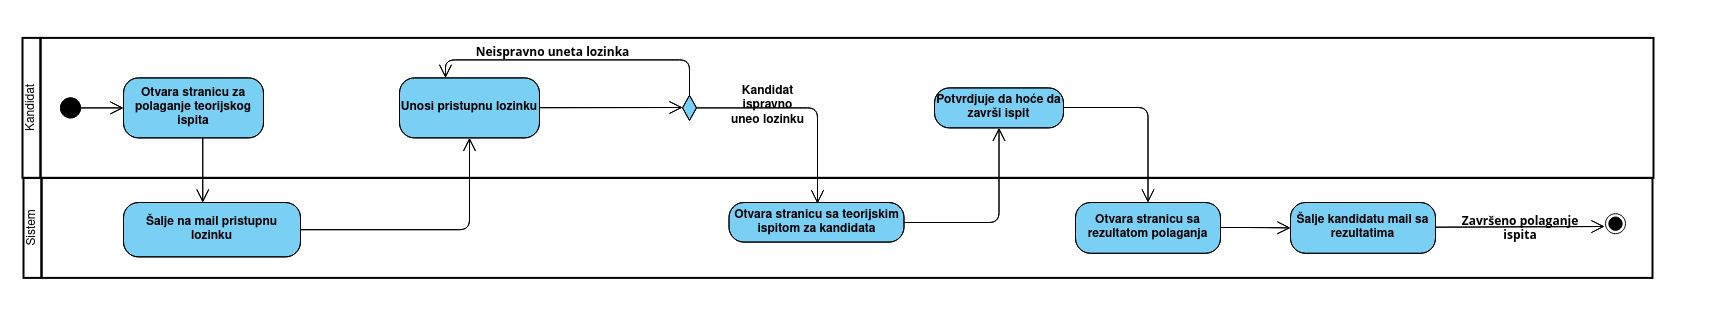
\includegraphics[width=140mm, height=70mm]{Diagrams/polaganje teorijskog ispita.png}
  \end{center}
  \caption {Dijagram aktivnosti - polaganje teorijskog ispita}
  \label{activity_polaganje_teorije}

\end{figure}
